\documentclass[11pt]{article}
\usepackage{amsmath,amssymb,amsthm}
\usepackage{fancyhdr}
\usepackage{tikz-qtree}
\usepackage{enumerate}
\usepackage{graphicx}

% margins
\usepackage[vmargin=1in,hmargin=1.5in]{geometry}

% Config
%%%%%%%%%%%%%%%%%%%%%%%%%%%%%%%%%%%
\newcommand{\ass}{1}
\newcommand{\name}{Connor Taffe}
\newcommand{\tno}{3742} % last 4 digits of T number.
%%%%%%%%%%%%%%%%%%%%%%%%%%%%%%%%%%%

\title{
	$A_{\ass}$ \\
	{\large Assignment \ass\\
	CS 3482; Professor Tang}
}
\author{
	\name. T no. \tno
}

% TODO: Remember to update this.
\date{April $21^{\text{st}}$, 2015}

\pagestyle{fancy}
\rhead{Homework \ass}
\lhead{{\name}. T no. \tno}

\begin{document}
\maketitle

\section{Question}

Draw the circuit in LogicWorks to implement the Boolean function:
\begin{figure}[h]
\[
	f(a,b,c,d) = (a'+b)'c+d(b'+ac)
\]
\caption{Given boolean function $f$}
\label{eqbool}
\end{figure}

\begin{figure}[h]
	\centering
	\Tree [.$+$ [.$*$ [.$+$ [.$`$ $a$ ] $b$ ] $c$ ] [.$*$ $d$ [.+ [.$`$ $b$ ] [.$*$ $a$ $c$ ] ] ] ]
\caption{Parse tree of figure \ref{eqbool}}
\label{eqboolparsetree}
\end{figure}

\begin{figure}[h]
	\centering
	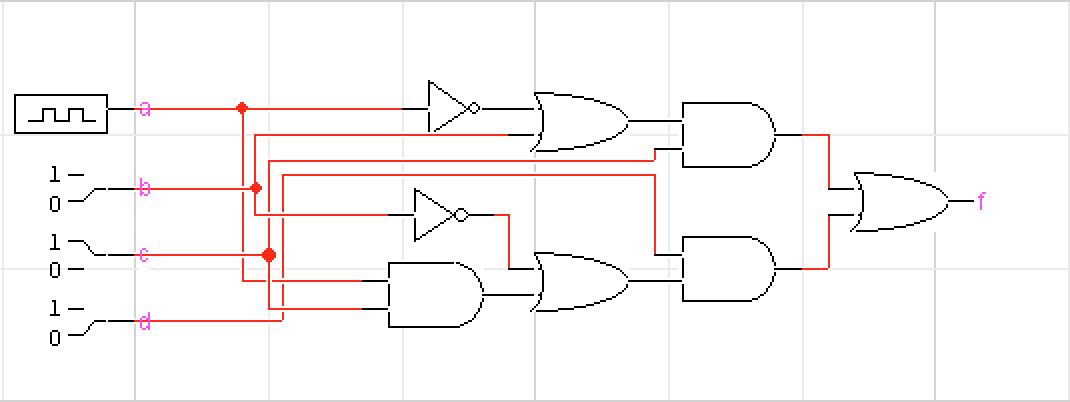
\includegraphics[width=200pt]{nc}
	\caption{LogicWorks implementation of $f$}
	\label{eqboollw}
\end{figure}

\begin{figure}[h]
	\centering
	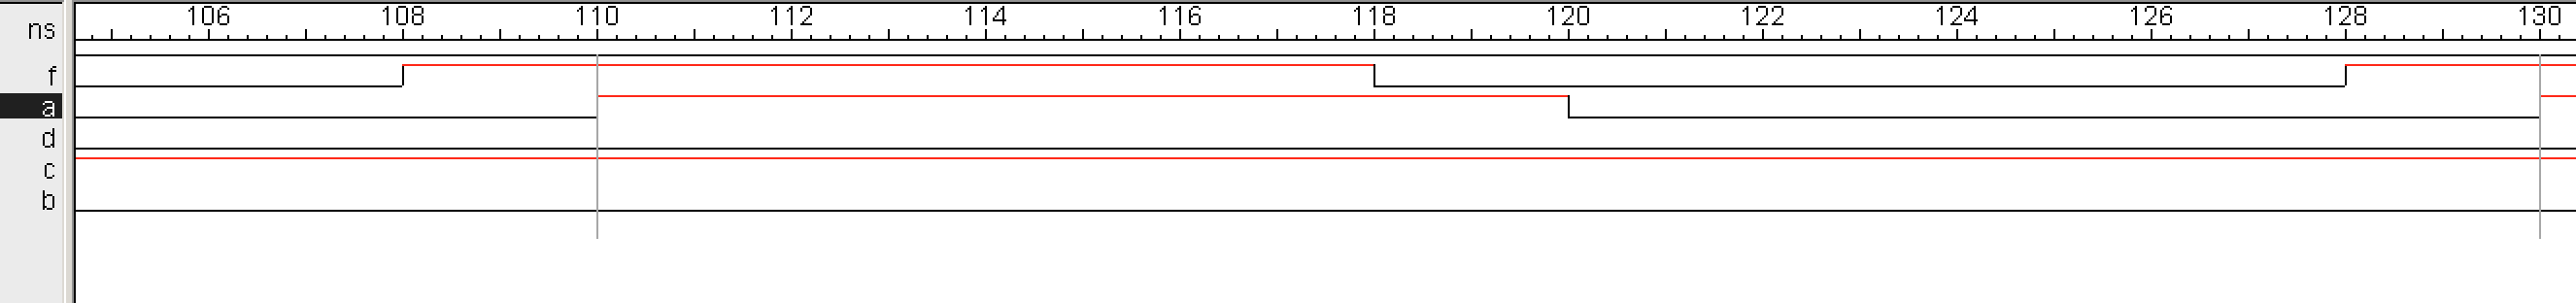
\includegraphics[width=300pt]{nc-wave}
	\caption{LogicWorks implementation of $f$, waveforms}
	\label{eqboollw-wave}
\end{figure}

\begin{enumerate}[(a)]
	\item{
		Figure \ref{eqboolparsetree} shows the structure of a naive circuit implementation. Figure \ref{eqboollw} shows the LogicWorks implementation of the circuit.
	}
	\item{
		I observed an 18ns delay between $a$ and $f$ (shown in figure \ref{eqboollw-wave}). This is because the gate delays between $a$ and $f$ accumulate.
	}
\end{enumerate}

\section{Question}

Simplify the same Boolean function in figure \ref{eqbool} to be the sum of its minterms by obtaining is truth table first.

\begin{figure}[h]
	\centering
	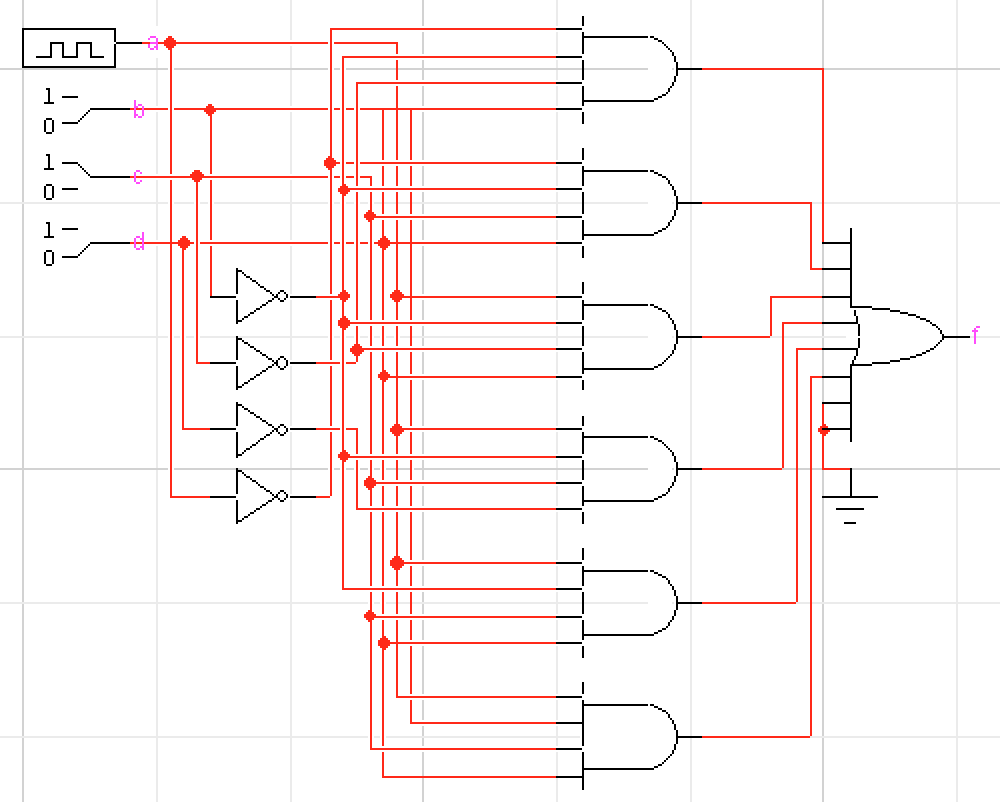
\includegraphics[width=200pt]{mtc}
	\caption{LogicWorks implementation of $f_{\text{minterm}}$}
	\label{eqboollw2}
\end{figure}

\begin{figure}[h]
	\centering
	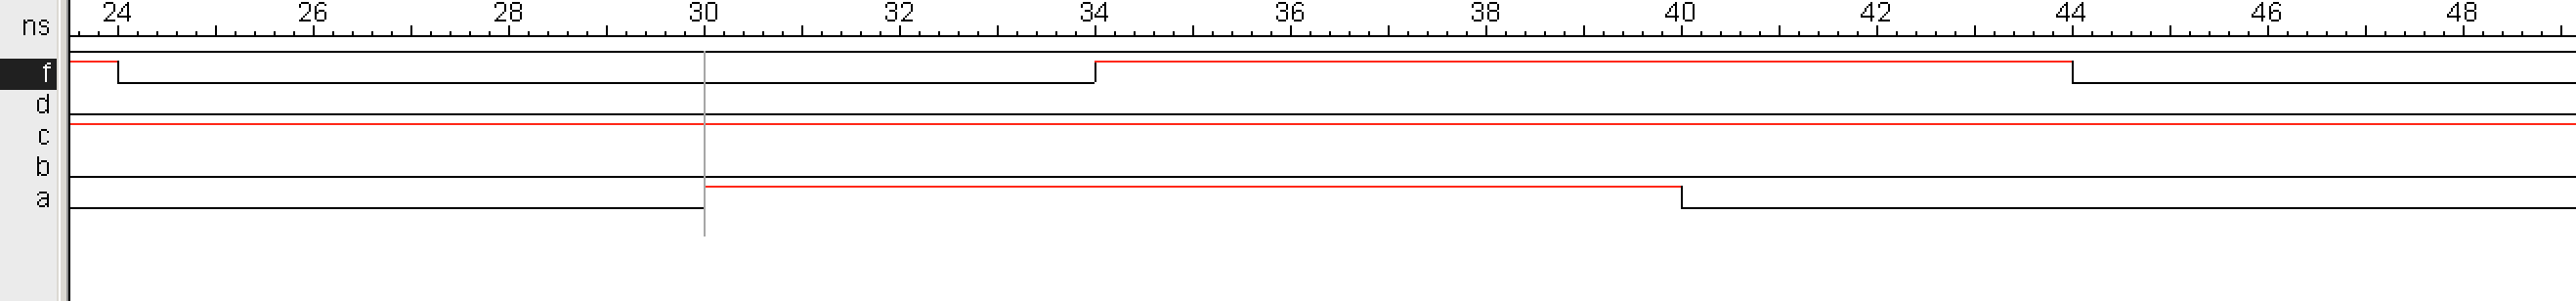
\includegraphics[width=300pt]{mtc-wave}
	\caption{LogicWorks implementation of $f_{\text{minterm}}$, waveforms}
	\label{eqboollw-wave2}
\end{figure}

\begin{table}[h]
\centering
\begin{tabular}{lllllllllllll}
	$a$ & $b$ & $c$ & $d$ & $a'$ & $a'+b$ & $(a'+b)'$ & $(a'+b)'c$ & $ac$ & $b'$ & $b'+ac$ & $d(b'+ac)$ & $f$ \\ \hline
	0 & 0 & 0 & 0 & 1 & 1 & 0 & 0 & 0 & 1 & 1 & 0 & 0 \\
	0 & 0 & 0 & 1 & 1 & 1 & 0 & 0 & 0 & 1 & 1 & 1 & 1 \\
	0 & 0 & 1 & 0 & 1 & 1 & 0 & 0 & 0 & 1 & 1 & 0 & 0 \\
	0 & 0 & 1 & 1 & 1 & 1 & 0 & 0 & 0 & 1 & 1 & 1 & 1 \\
	0 & 1 & 0 & 0 & 1 & 1 & 0 & 0 & 0 & 0 & 0 & 0 & 0 \\
	0 & 1 & 0 & 1 & 1 & 1 & 0 & 0 & 0 & 0 & 0 & 0 & 0 \\
	0 & 1 & 1 & 0 & 1 & 1 & 0 & 0 & 0 & 0 & 0 & 0 & 0 \\
	0 & 1 & 1 & 1 & 1 & 1 & 0 & 0 & 0 & 0 & 0 & 0 & 0 \\
	1 & 0 & 0 & 0 & 0 & 0 & 1 & 0 & 0 & 1 & 1 & 0 & 0 \\
	1 & 0 & 0 & 1 & 0 & 0 & 1 & 0 & 0 & 1 & 1 & 1 & 1 \\
	1 & 0 & 1 & 0 & 0 & 0 & 1 & 1 & 1 & 1 & 1 & 0 & 1 \\
	1 & 0 & 1 & 1 & 0 & 0 & 1 & 1 & 1 & 1 & 1 & 1 & 1 \\
	1 & 1 & 0 & 0 & 0 & 1 & 0 & 0 & 0 & 0 & 0 & 0 & 0 \\
	1 & 1 & 0 & 1 & 0 & 1 & 0 & 0 & 0 & 0 & 0 & 0 & 0 \\
	1 & 1 & 1 & 0 & 0 & 1 & 0 & 0 & 1 & 0 & 1 & 0 & 0 \\
	1 & 1 & 1 & 1 & 0 & 1 & 0 & 0 & 1 & 0 & 1 & 1 & 1
\end{tabular}
\caption{Truth table for $f$ as described in figure \ref{eqbool}}
\label{truthtable}
\end{table}

\begin{figure}[h]
	\centering
	\Tree [.$+$
		[.$*$ [.$`$ $a$ ] [.$`$ $b$ ] [.$`$ $c$ ] $d$ ]
		[.$*$ [.$`$ $a$ ] [.$`$ $b$ ] $c$ $d$ ]
		[.$*$ $a$ [.$`$ $b$ ] [.$`$ $c$ ] $d$ ]
		[.$*$ $a$ [.$`$ $b$ ] $c$ [.$`$ $d$ ] ]
		[.$*$ $a$ [.$`$ $b$ ] $c$ $d$ ]
		[.$*$ $a$ $b$ $c$ $d$ ]
	]
\caption{Parse tree of minterms of $f$}
\label{mintermparsetree}
\end{figure}

\begin{enumerate}[(a)]
	\item{
		Figure \ref{truthtable} shows the truth table for the function.
	}
	\item{$f_{\text{minterm}} = a'b'c'd + a'b'cd + ab'c'd + ab'cd' + ab'cd + abcd$}
	\item{Figure \ref{mintermparsetree} shows the parse tree and thusly the gate implementation of the minterms of $f$. The LogicWorks circuit is represented in figure \ref{eqboollw2}.}
	\item{I observed a delay of 4ns between $a$ and $f$ (shown in figure \ref{eqboollw-wave2}). This is because the delays between $a$ and $f$ accumulate as in the naive implementation, but less so as there is a maximum of three gates in the path beween $a$ and $f$.}
\end{enumerate}

\section{Question}

\begin{figure}[h]
	\centering
	\Tree [.$y_0$ [.$*$ [.$`$ $x_1$ ] [.$`$ $x_0$ ] $E$ ] ]
	\Tree [.$y_1$ [.$*$ [.$`$ $x_1$ ] $x_0$ $E$ ] ]
	\Tree [.$y_2$ [.$*$ $x_1$ [.$`$ $x_0$ ] $E$ ] ]
	\Tree [.$y_3$ [.$*$ $x_1$ $x_0$ $E$ ] ]

\caption{Parse trees of 2-to-4 decoder with an active-high enable $E$}
\label{2to4parsetree}
\end{figure}

\begin{figure}[h]
	\centering
	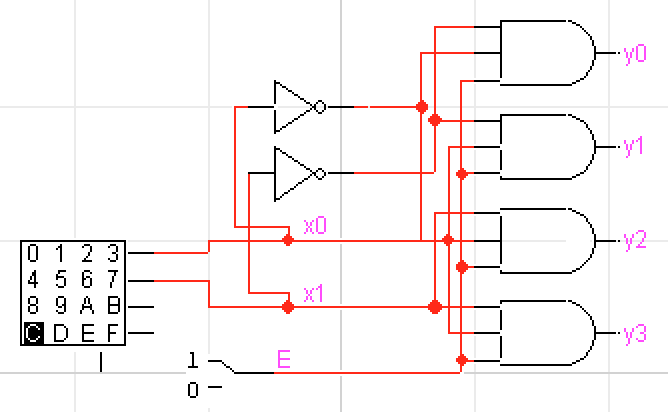
\includegraphics[width=200pt]{2to4testc}
	\caption{Internal circuit of a 2-4 decoder; being tested.}
	\label{2to4testc}
\end{figure}

\begin{figure}[h]
	\centering
	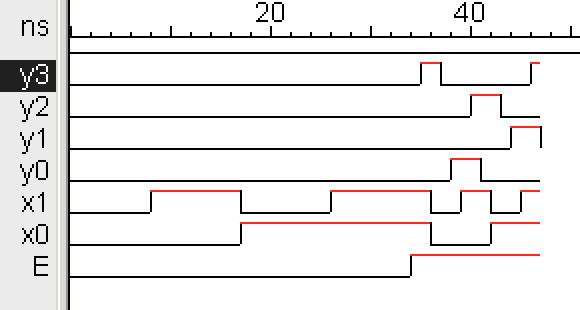
\includegraphics[width=100pt]{2to4test}
	\caption{Test waveform output of a 2-4 decoder.}
	\label{2to4test}
\end{figure}

\begin{figure}[h]
	\centering
	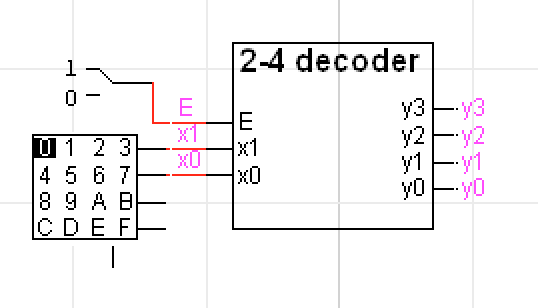
\includegraphics[width=200pt]{2to4pkgtestc}
	\caption{Internal circuit of a 2-4 decoder (packaged); being tested.}
	\label{2to4pkgtestc}
\end{figure}

\begin{figure}[h]
	\centering
	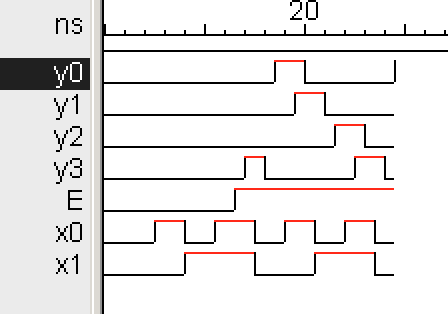
\includegraphics[width=100pt]{2to4pkgtest}
	\caption{Test waveform output of a 2-4 decoder (packaged).}
	\label{2to4pkgtest}
\end{figure}

\begin{enumerate}[(a)]
	\item{Figure \ref{2to4parsetree} shows the trees of a 2-to-4 decoder with an active-high enable $E$. Testing is shown in figure \ref{2to4test}, and the tested circuit LogicWorks implementation is shown in figure \ref{2to4testc}.}
	\item{Testing is shown in figure \ref{2to4pkgtest}, and the tested circuit LogicWorks packaged implementation is shown in figure \ref{2to4pkgtestc}.}
\end{enumerate}

\section{Question}

\begin{figure}[h]
	\centering
	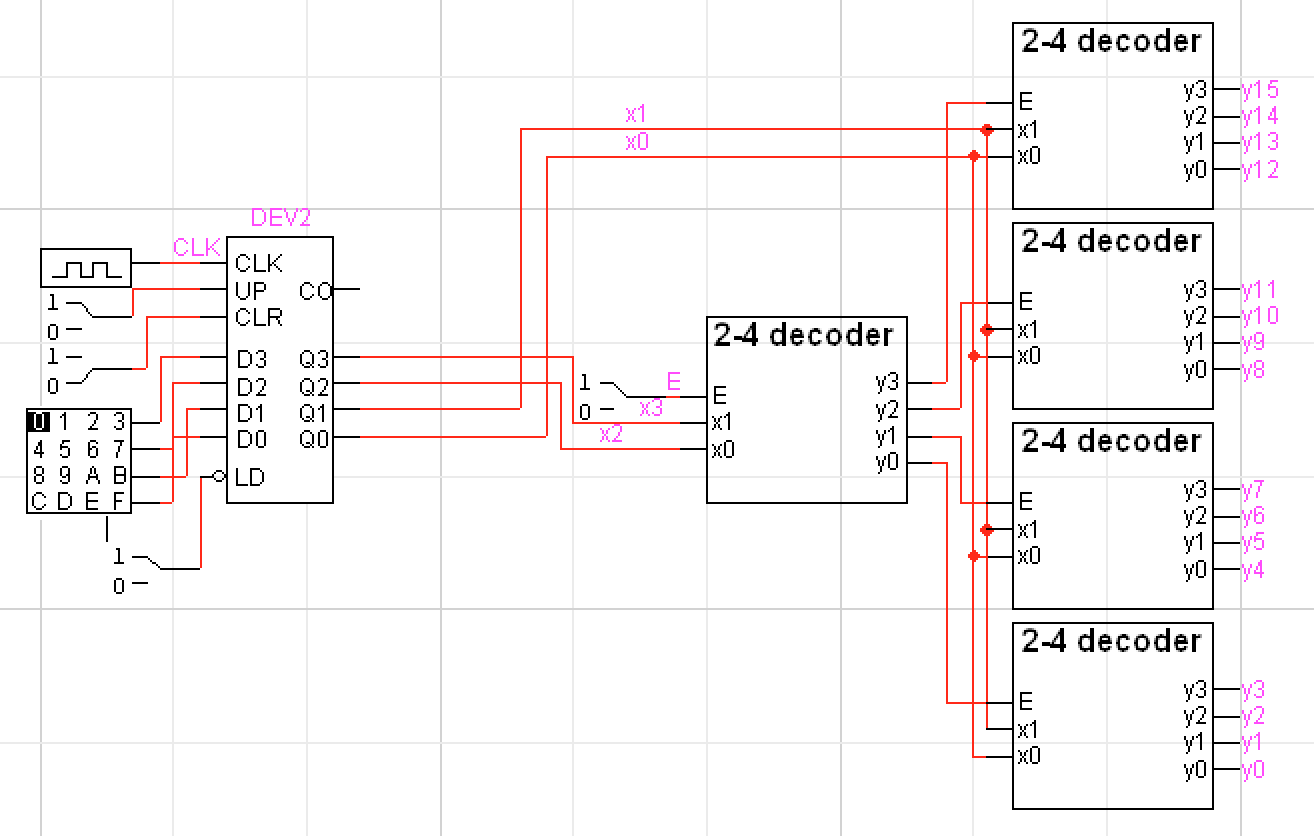
\includegraphics[width=300pt]{4to16testc}
	\caption{Internal circuit of a 4-16 decoder; being tested.}
	\label{4to16testc}
\end{figure}

\begin{figure}[h]
	\centering
	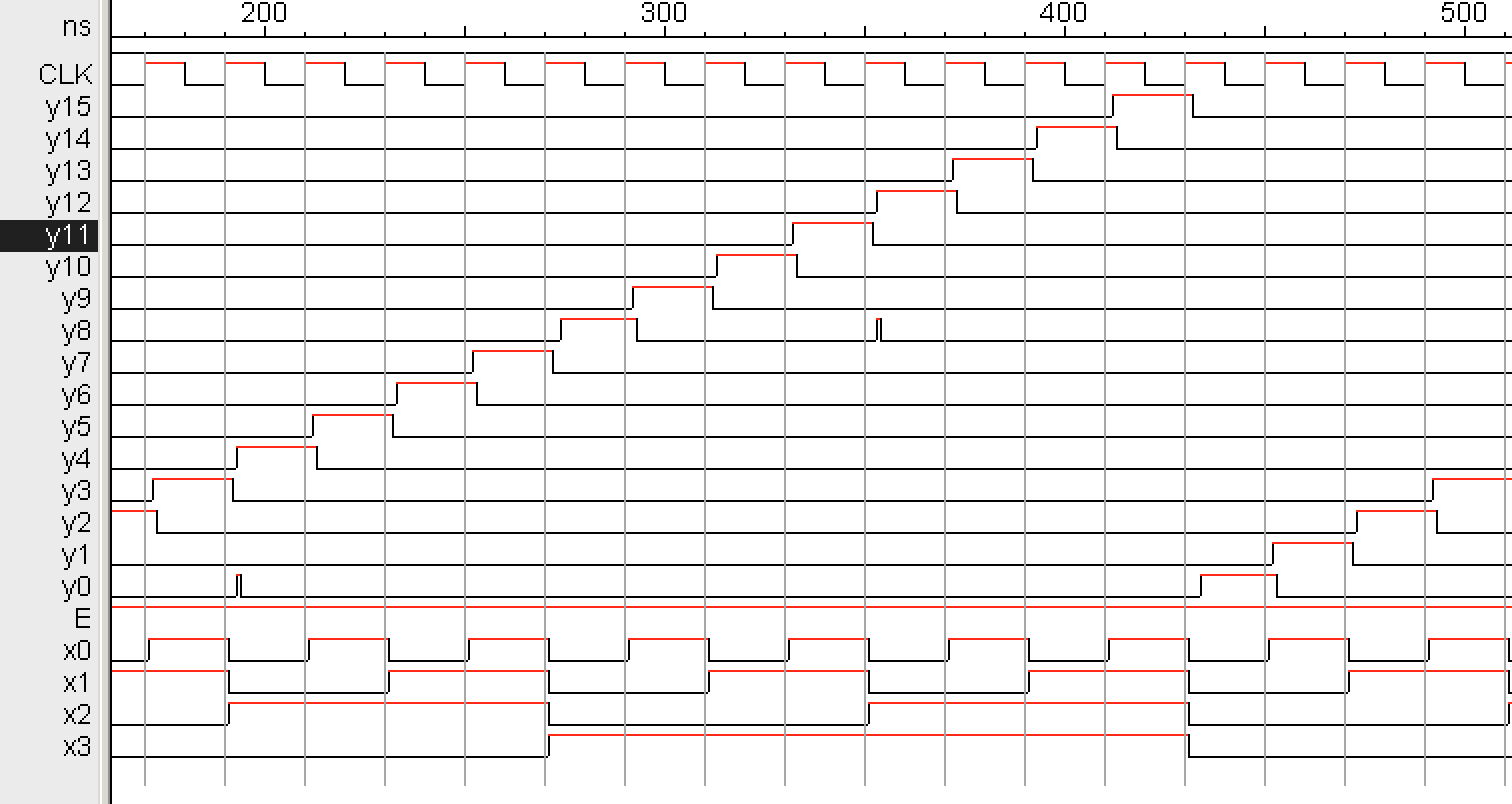
\includegraphics[width=300pt]{4to16test}
	\caption{Test waveform output of a 4-16 decoder.}
	\label{4to16test}
\end{figure}

\begin{figure}[h]
	\centering
	% zeroth 2-4 decoder
	\Tree [.$y_{u,0}$ [.$*$ [.$`$ $x_1$ ] [.$`$ $x_0$ ] $E$ ] ]
	\Tree [.$y_{u,1}$ [.$*$ [.$`$ $x_1$ ] $x_0$ $E$ ] ]
	\Tree [.$y_{u,2}$ [.$*$ $x_1$ [.$`$ $x_0$ ] $E$ ] ]
	\Tree [.$y_{u,3}$ [.$*$ $x_1$ $x_0$ $E$ ] ]

	\Tree [.$y_{0}$ [.$*$ [.$`$ $x_3$ ] [.$`$ $x_2$ ] $y_{u,0}$ ] ]
	\Tree [.$y_{1}$ [.$*$ [.$`$ $x_3$ ] $x_2$ $y_{u,0}$ ] ]
	\Tree [.$y_{2}$ [.$*$ $x_3$ [.$`$ $x_2$ ] $y_{u,0}$ ] ]
	\Tree [.$y_{3}$ [.$*$ $x_3$ $x_2$ $y_{u,0}$ ] ]

	\Tree [.$y_{4}$ [.$*$ [.$`$ $x_3$ ] [.$`$ $x_2$ ] $y_{u,1}$ ] ]
	\Tree [.$y_{5}$ [.$*$ [.$`$ $x_3$ ] $x_2$ $y_{u,1}$ ] ]
	\Tree [.$y_{6}$ [.$*$ $x_3$ [.$`$ $x_2$ ] $y_{u,1}$ ] ]
	\Tree [.$y_{7}$ [.$*$ $x_3$ $x_2$ $y_{u,1}$ ] ]

	\Tree [.$y_{8}$ [.$*$ [.$`$ $x_3$ ] [.$`$ $x_2$ ] $y_{u,2}$ ] ]
	\Tree [.$y_{9}$ [.$*$ [.$`$ $x_3$ ] $x_2$ $y_{u,2}$ ] ]
	\Tree [.$y_{10}$ [.$*$ $x_3$ [.$`$ $x_2$ ] $y_{u,2}$ ] ]
	\Tree [.$y_{11}$ [.$*$ $x_3$ $x_2$ $y_{u,2}$ ] ]

	\Tree [.$y_{12}$ [.$*$ [.$`$ $x_3$ ] [.$`$ $x_2$ ] $y_{u,3}$ ] ]
	\Tree [.$y_{13}$ [.$*$ [.$`$ $x_3$ ] $x_2$ $y_{u,3}$ ] ]
	\Tree [.$y_{14}$ [.$*$ $x_3$ [.$`$ $x_2$ ] $y_{u,3}$ ] ]
	\Tree [.$y_{15}$ [.$*$ $x_3$ $x_2$ $y_{u,3}$ ] ]

\caption{Parse trees of 4-to-16 decoder with an active-high enable $E$. For convenience and space the first line depicts the inner 2-to-4 decoder for the first two bits, denoted with subscript $u$.}
\label{4to16parsetree}
\end{figure}

\begin{enumerate}[(a)]
	\item{Five, one for the first two bits, and four for each of the four minterms of the first two bits.}
	\item{Figure \ref{4to16parsetree} shows the parse trees of a 4-to-16 decoder built only using 2-to-4 decoders. The parse tree describes the gate diagram. The LogicWorks implementation can be seen in figure \ref{4to16testc}.}
	\item{Figure \ref{4to16test} shows the waveform.}
\end{enumerate}

\end{document}
